\documentclass[11pt]{amsart}
\usepackage{geometry}                % See geometry.pdf to learn the layout options. There are lots.
\geometry{letterpaper}                   % ... or a4paper or a5paper or ... 
%\geometry{landscape}                % Activate for for rotated page geometry
%\usepackage[parfill]{parskip}    % Activate to begin paragraphs with an empty line rather than an indent
\usepackage{graphicx}
\usepackage{amssymb}
\usepackage{epstopdf}
\usepackage{tikz}
\usetikzlibrary{3d,shapes,snakes,positioning}
\DeclareGraphicsRule{.tif}{png}{.png}{`convert #1 `dirname #1`/`basename #1 .tif`.png}

\begin{document}


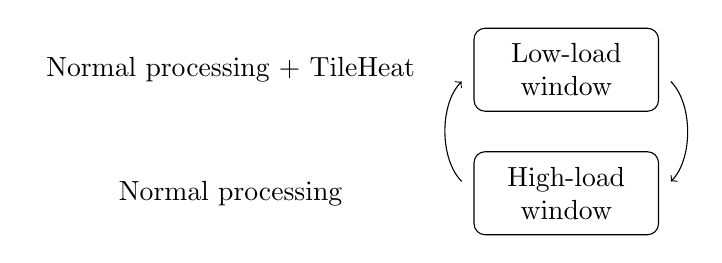
\begin{tikzpicture}[node distance=0.5cm, auto]

\tikzstyle{kasse}=[rectangle, rounded corners, draw=black, text width=6em, minimum height=3em, text centered]
\tikzstyle{tomkasse}=[text width=14em, minimum height=3em, text centered]
\tikzstyle{pil}=[->, shorten >=6pt, shorten <=6pt]

%\draw[<->] (3,1) -- (3,-2.5);
%\node at (5,-0.8) {Time period};

\node[kasse] (low) {Low-load window};
\node[tomkasse, left=of low] (tasklow) {Normal processing + TileHeat};

\node[kasse, below=of low] (high) {High-load window};
\node[tomkasse, left=of high] (taskhigh) {Normal processing};


\draw[pil, bend left=45] (low.east) to (high.east);
\draw[pil, bend left=45] (high.west) to (low.west);

\end{tikzpicture}

\end{document}  